\documentclass[11pt,a4paper]{article}
\usepackage[margin=2.5cm]{geometry}
\usepackage{amsmath,amssymb}
\usepackage{booktabs}
\usepackage{siunitx}
\usepackage{pgfplots}
\usepackage{graphicx}
\usepackage{hyperref}
\pgfplotsset{compat=1.17}
\sisetup{per-mode=symbol}

\newcommand{\VR}{\vec V_{\!R}}
\newcommand{\VP}{\vec V_{\!P}}
\newcommand{\Atop}{A_{\mathrm{top}}}
\newcommand{\Af}{A_{\mathrm{f}}}
\newcommand{\As}{A_{\mathrm{s}}}
\newcommand{\Ucrit}{U_{\mathrm{crit}}}

\title{Directional Rain Exposure: A Flux-Based Vectorial Model,\\ Realistic Bodies, Airflow and a Field Test}
\author{Alberto Valdes Rey}
\date{October 2026}

\begin{document}
\maketitle

\begin{abstract}
We model how much rain a person collects while moving a distance $\Delta L$ through rain driven by wind of arbitrary direction. The model rests on one principle: the volume flux onto a surface element equals the liquid water content times the component of the rain velocity \emph{relative to the person} along the inward normal. For a box-shaped body this gives a closed form with top, front, back and side contributions. The optimal speed follows from it. In still air, in a headwind, or in a weak tailwind, you should move as fast as possible. When the tailwind component exceeds a critical value $\Ucrit=(\Atop v_t+\As|U_y|)/\Af$ (about \SI{1}{\metre\per\second} for an adult), the best speed is exactly the tailwind speed. We validate the closed form against a three-dimensional Monte Carlo simulation of individual drops; all cases agree within statistical error. We then go beyond the box. A human-shaped body, with posture and lean that change with speed, collects 20--50\% less than the box, mainly because its frontal silhouette is about \SI{0.5}{m^2} rather than \SI{0.79}{m^2}. Airflow around the body deflects small drops; we trace drops through a potential-flow field and find that typical rain loses 10--30\% of its wind-driven catch, and drizzle 50--90\%. For a runner, limbs shield the chest from near-vertical rain, so overtaking a strong tailwind costs little and the sharp optimum softens. Finally, we design a field experiment with three absorbent pads whose ratio cancels rain intensity, and show by simulation that about 27 trials detect the predicted dip at the wind speed. Typical exposures over \SI{200}{m} are a few tens of millilitres.
\end{abstract}

\section{Introduction}
Whether to walk or run in the rain is a classic problem in elementary physics \cite{holden1995,ehrmann2011,bocci2012}. The answer depends on the wind, so a correct treatment must be vectorial. We build the model from a single flux principle (Section~\ref{sec:flux}). We then derive closed forms for a box-shaped body (Section~\ref{sec:box}), find the optimal speed (Section~\ref{sec:opt}), and validate everything against a particle simulation (Section~\ref{sec:mc}). Sections~\ref{sec:aero}--\ref{sec:combined} replace the box with a human body and add aerodynamic deflection of drops, and Section~\ref{sec:exp} designs a field experiment to test the central prediction.

\section{The rain field}\label{sec:rain}
Take $x$ along the direction of travel, $z$ upward, and $y$ to the walker's left. Drops fall at their terminal velocity $v_t$ and are carried horizontally by a wind of speed $U$ blowing toward azimuth $\varphi$ ($\varphi=0$: tailwind; $\varphi=\pi$: headwind; $\varphi=\pi/2$: crosswind):
\begin{equation}
\VR=(U_x,\,U_y,\,-v_t)=(U\cos\varphi,\;U\sin\varphi,\;-v_t),\qquad \VP=(v,0,0).
\end{equation}
The wind adds a horizontal component and leaves the fall speed unchanged; the rain angle follows from $\tan\theta=U/v_t$.

\paragraph{Terminal velocity.} We use the fit of Atlas et al.\ \cite{atlas1973} to the measurements of Gunn and Kinzer \cite{gunn1949}:
\begin{equation}
v_t(D)\approx 9.65-10.3\,e^{-0.6D}\ \si{\metre\per\second},\qquad D \text{ in mm},
\end{equation}
which gives \SI{2.0}{\metre\per\second} at \SI{0.5}{mm}, \SI{4.0}{\metre\per\second} at \SI{1}{mm}, \SI{6.55}{\metre\per\second} at \SI{2}{mm} and \SI{8.0}{\metre\per\second} at \SI{3}{mm}.

\paragraph{Liquid water content.} Let $C$ be the volume of liquid water per unit volume of air. The rainfall rate $R$ is the vertical flux of that water through a horizontal plane, $R=C\,v_t$. Hence
\begin{equation}
C=\frac{R}{v_t}.
\end{equation}
For $R=\SI{5}{mm/h}$ and $D=\SI{2}{mm}$, this gives $C=\num{2.1e-7}$ (\SI{0.21}{g/m^3}, or \SI{2.1e-4}{L/m^3}), about 51 drops per cubic metre. Table~\ref{tab:rain} lists other rates. (A drop-size distribution such as Marshall--Palmer \cite{marshall1948} replaces $C$ and $v_t$ by sums over size classes; the structure of the model is unchanged.)

\begin{table}[h]\centering
\caption{Liquid water content for \SI{2}{mm} drops ($v_t=\SI{6.55}{m/s}$).}\label{tab:rain}
\begin{tabular}{lccc}\toprule
Rain & $R$ (mm/h) & $C$ (g/m$^3$) & drops/m$^3$\\\midrule
Light & 1 & 0.042 & 10\\
Moderate & 5 & 0.21 & 51\\
Heavy & 20 & 0.85 & 203\\
Very heavy & 50 & 2.1 & 506\\\bottomrule
\end{tabular}
\end{table}

\section{Flux principle}\label{sec:flux}
In the walker's rest frame, the rain moves with relative velocity
\begin{equation}
\vec u=\VR-\VP=(U_x-v,\;U_y,\;-v_t).
\end{equation}
A surface element $dA$ with outward normal $\hat n$ is hit only if the rain moves into it, i.e.\ if $\vec u\cdot\hat n<0$. The volume of water it receives per unit time is $C\max(0,-\vec u\cdot\hat n)\,dA$. Integrating over the body and over the trip duration $T=\Delta L/v$ gives
\begin{equation}\label{eq:general}
K=C\,\frac{\Delta L}{v}\oint_{\text{body}}\max\!\big(0,-\vec u\cdot\hat n\big)\,dA
= C\,\frac{\Delta L}{v}\,|\vec u|\,A_\perp(\hat u),
\end{equation}
where $A_\perp(\hat u)$ is the silhouette area seen by the incoming rain. The surface integral is valid for convex bodies; the silhouette form is valid for \emph{any} body, because each drop is caught by the first surface it meets, so parts shaded by other parts are automatically excluded. The result is easy to picture. $K$ is the water inside the oblique tube that the body's silhouette sweeps through the rain field, which has length $|\vec u|\,T$ and cross-section $A_\perp$.

\section{Box-shaped body}\label{sec:box}
Model the body as a box of height $h$, shoulder breadth $b$ and chest-to-back thickness $d$. The relevant areas are projected areas, not skin area:
\begin{equation}
\Atop=bd,\qquad \Af=A_{\mathrm{back}}=bh,\qquad \As=dh .
\end{equation}
For $h=\SI{1.75}{m}$, $b=\SI{0.45}{m}$ and $d=\SI{0.25}{m}$, this gives $\Atop=\SI{0.113}{m^2}$, $\Af=\SI{0.788}{m^2}$ and $\As=\SI{0.438}{m^2}$. Applying \eqref{eq:general} face by face:
\begin{align}
K_{\mathrm{top}}&=C\,\Delta L\,\frac{\Atop\,v_t}{v},\\
K_{\mathrm{front}}&=C\,\Delta L\,\Af\,\frac{\max(0,\,v-U_x)}{v},\\
K_{\mathrm{back}}&=C\,\Delta L\,\Af\,\frac{\max(0,\,U_x-v)}{v},\\
K_{\mathrm{side}}&=C\,\Delta L\,\frac{\As\,|U_y|}{v}.
\end{align}
At most one of front and back is wet; which one depends only on the sign of $v-U_x$. Summing,
\begin{equation}\label{eq:box}
\boxed{K(v)=C\,\Delta L\left[\frac{\Atop v_t+\As|U_y|}{v}+\Af\left|1-\frac{U_x}{v}\right|\right]}
\end{equation}
Units: $[C\,\Delta L\,A]=\si{m^3}$, and every bracketed factor is dimensionless.

\paragraph{Remarks.}
\begin{itemize}
\item \emph{Still air} ($U=0$): $K=C\,\Delta L\,(\Atop v_t/v+\Af)$. The front term $C\,\Delta L\,\Af$ does not depend on speed, because the walker sweeps out the same volume of air whatever the pace.
\item \emph{Infinite speed:} $K\to C\,\Delta L\,\Af$. This is a hard lower bound in still air or a headwind.
\item \emph{Headwind} ($U_x<0$): the front sees relative speed $v+|U_x|$. The headwind \emph{increases} exposure compared with still air.
\item \emph{Tailwind} ($U_x>0$): the back is wet while you are slower than the wind, and the front is wet once you overtake it.
\end{itemize}

\section{Optimal speed}\label{sec:opt}
Write $a=\Atop v_t+\As|U_y|>0$. On $0<v<U_x$, $K=C\Delta L[(a+\Af U_x)/v-\Af]$, which decreases in $v$. On $v>U_x$, $K=C\Delta L[(a-\Af U_x)/v+\Af]$, which decreases only if $a>\Af U_x$. Hence, with $v\le v_{\max}$:
\begin{equation}
v^\ast=\begin{cases}U_x, & U_x>\Ucrit \text{ and } U_x\le v_{\max},\\ v_{\max}, & \text{otherwise,}\end{cases}
\qquad
\Ucrit=\frac{\Atop v_t+\As|U_y|}{\Af}.
\end{equation}
Without crosswind, $\Ucrit=(d/h)\,v_t\approx 0.14\,v_t\approx\SI{0.94}{m/s}$ for \SI{2}{mm} drops. A tailwind stronger than a gentle breeze therefore makes \emph{matching the wind} optimal. At $v=U_x$ only the top (and possibly a side) is wet, and $K_{\min}=C\,\Delta L\,a/U_x$. This agrees with the result of Bocci \cite{bocci2012}: ``always run'' is false in this regime.

\section{Results}
Table~\ref{tab:results} uses $R=\SI{5}{mm/h}$, $D=\SI{2}{mm}$, $\Delta L=\SI{200}{m}$, walking at \SI{1.4}{m/s}, running at \SI{3.3}{m/s} and sprinting at \SI{6}{m/s}. Figure~\ref{fig:curves} shows $K(v)$ for four wind conditions.

\begin{table}[h]\centering
\caption{Water collected over \SI{200}{m} (mL). ``Walk breakdown'' lists top/front/back/side.}\label{tab:results}
\begin{tabular}{lcccccc}\toprule
Wind & walk breakdown & walk & run & sprint & $v^\ast$ (m/s) & $K(v^\ast)$\\\midrule
Still air & 22.3/33.4/0/0 & 55.7 & 42.9 & 38.6 & max & 38.6\\
Headwind 3 m/s & 22.3/105.0/0/0 & 127.3 & 73.2 & 55.3 & max & 55.3\\
Tailwind 1 m/s & 22.3/9.5/0/0 & 31.9 & 32.8 & 33.0 & 1.0 & 31.3\\
Tailwind 2 m/s & 22.3/0/14.3/0 & 36.6 & 22.6 & 27.5 & 2.0 & 15.6\\
Tailwind 5 m/s & 22.3/0/85.9/0 & 108.2 & 26.7 & 10.8 & 5.0 & 6.2\\
Crosswind 3 m/s & 22.3/33.4/0/39.8 & 95.5 & 59.8 & 47.9 & max & 47.9\\\bottomrule
\end{tabular}
\end{table}

Three conclusions follow:
\begin{enumerate}
\item The amounts are tens of millilitres, roughly a few spoonfuls, which matches everyday experience.
\item Headwind is the \emph{worst} direction, because the front meets the rain at $v+|U_x|$.
\item With a \SI{2}{m/s} tailwind, running at \SI{3.3}{m/s} beats walking, but jogging at exactly \SI{2}{m/s} beats both (\SI{15.6}{mL}). With a \SI{1}{m/s} tailwind, walking and running are nearly equal.
\end{enumerate}

\begin{figure}[h]\centering
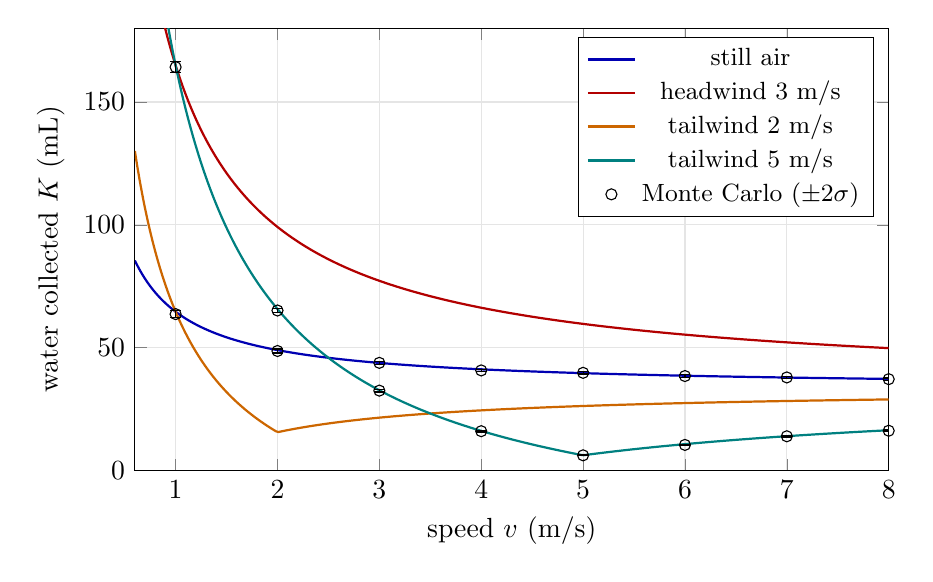
\begin{tikzpicture}
% K(v) = C ΔL [a/v + Af |1 - Ux/v|] in mL; C ΔL = 42.424 mL/m², a = Atop·vt = 0.73662 m³/s per (m/s)
\begin{axis}[width=0.92\textwidth,height=7.2cm,xmin=0.6,xmax=8,ymin=0,ymax=180,
  xlabel={speed $v$ (m/s)},ylabel={water collected $K$ (mL)},grid=major,grid style={gray!20},
  legend style={font=\small,at={(0.98,0.98)},anchor=north east},domain=0.6:8,samples=300]
\addplot[blue!70!black,thick] {42.424*(0.73662/x + 0.7875)};
\addlegendentry{still air}
\addplot[red!70!black,thick] {42.424*(0.73662/x + 0.7875*abs(1+3/x))};
\addlegendentry{headwind 3 m/s}
\addplot[orange!80!black,thick] {42.424*(0.73662/x + 0.7875*abs(1-2/x))};
\addlegendentry{tailwind 2 m/s}
\addplot[teal,thick] {42.424*(0.73662/x + 0.7875*abs(1-5/x))};
\addlegendentry{tailwind 5 m/s}
\addplot[only marks,mark=o,mark size=2pt,black,error bars/.cd,y dir=both,y explicit] coordinates {
(1,63.68) +- (0,1.35) (2,48.67) +- (0,0.83) (3,43.85) +- (0,0.65) (4,40.77) +- (0,0.54)
(5,39.79) +- (0,0.48) (6,38.48) +- (0,0.47) (7,37.91) +- (0,0.46) (8,37.21) +- (0,0.46)};
\addlegendentry{Monte Carlo ($\pm2\sigma$)}
\addplot[only marks,mark=o,mark size=2pt,black,forget plot,error bars/.cd,y dir=both,y explicit] coordinates {
(1,164.18) +- (0,2.16) (2,65.15) +- (0,0.96) (3,32.55) +- (0,0.56) (4,16.04) +- (0,0.34)
(5,6.22) +- (0,0.19) (6,10.46) +- (0,0.24) (7,13.97) +- (0,0.28) (8,16.23) +- (0,0.30)};
\end{axis}
\end{tikzpicture}
\caption{$K(v)$ from \eqref{eq:box} for $R=\SI{5}{mm/h}$, $D=\SI{2}{mm}$ and $\Delta L=\SI{200}{m}$. Circles show Monte Carlo estimates for still air and for a \SI{5}{m/s} tailwind. The tailwind curve has a sharp minimum at $v=U_x$.}\label{fig:curves}
\end{figure}

\section{Monte Carlo validation}\label{sec:mc}
The accompanying simulator (\texttt{src/rain-model.js}, \texttt{src/simulation.html}) checks \eqref{eq:box} without assuming it. It works as follows:
\begin{itemize}
\item Drops are tracked as points in a 3D window around the body, in the walker's rest frame, where they move with velocity $\vec u$. Each simulated parcel represents a known number of real drops.
\item The upstream field is kept exactly uniform. New parcels enter through every inflow face of the window at rate $n\,|\vec u\cdot\hat n|\,A_{\text{face}}$, at a uniformly random point and instant within the step. Parcels leaving the window or reaching the ground are removed.
\item Each step's displacement is tested against the body box with the slab method. A hit is credited to the face the segment actually enters, so drops cannot tunnel through the body and no tolerance-based guesswork is involved.
\item Hits are Poisson counts, so the $1\sigma$ uncertainty of a face total is $\sqrt{N}$ times the water represented by one parcel.
\end{itemize}
Table~\ref{tab:mc} compares full \SI{200}{m} trips with the closed form. All twelve runs lie within $2.5\sigma$. Their mean deviation is consistent with zero, and twelve further runs of the still-air case with different seeds gave a mean $z=0.20$. The automated test suite (\texttt{tests/}) repeats such comparisons for each face separately.

\begin{table}[h]\centering
\caption{Closed form vs.\ Monte Carlo, full \SI{200}{m} trip, 4000 parcels in the window.}\label{tab:mc}
\begin{tabular}{lcccc}\toprule
Case & $v$ (m/s) & model (mL) & simulation (mL) & $z$\\\midrule
Still air & 1.4 & 55.73 & $56.12\pm0.24$ & $+1.6$\\
Still air & 3.3 & 42.88 & $42.97\pm0.21$ & $+0.4$\\
Headwind 3 m/s & 1.4 & 127.32 & $127.44\pm0.37$ & $+0.3$\\
Headwind 3 m/s & 3.3 & 73.25 & $73.10\pm0.28$ & $-0.5$\\
Tailwind 1 m/s & 1.4 & 31.87 & $32.01\pm0.18$ & $+0.8$\\
Tailwind 1 m/s & 3.3 & 32.75 & $33.08\pm0.19$ & $+1.7$\\
Tailwind 2 m/s & 1.4 & 36.64 & $36.62\pm0.20$ & $-0.1$\\
Tailwind 2 m/s & 3.3 & 22.63 & $22.97\pm0.16$ & $+2.2$\\
Tailwind 5 m/s & 1.4 & 108.23 & $107.41\pm0.34$ & $-2.4$\\
Tailwind 5 m/s & 3.3 & 26.68 & $26.68\pm0.17$ & $0.0$\\
Crosswind 3 m/s & 1.4 & 95.50 & $95.83\pm0.32$ & $+1.0$\\
Crosswind 3 m/s & 3.3 & 59.75 & $59.93\pm0.25$ & $+0.7$\\\bottomrule
\end{tabular}
\end{table}

\section{Airflow around the body}\label{sec:aero}
The box model assumes ballistic drops: every drop on a collision course hits. In reality the air moving past the walker, at relative velocity $\vec V=(U_x-v,\,U_y)$, bends around the body, and small drops follow it. We quantify this with a collection efficiency $\eta$, the fraction of drops on the capture tube that actually touch the body. Only the horizontally driven catch is affected, because the relative airflow is horizontal.

\paragraph{Method.} A horizontal cross-section of the torso is an ellipse with semi-axes $a=d/2=\SI{0.125}{m}$ (along the walking direction) and $b=\SI{0.225}{m}$ (half the shoulder breadth); a leg is a circle of radius \SI{0.065}{m}. The airflow is two-dimensional potential flow around the section, obtained by the Joukowski map $z=\zeta-k^2/\zeta$ from a circle of radius $R=(a+b)/2$ with $k^2=R(b-a)/2$; the complex potential is $W(\zeta)=\bar V\zeta+VR^2/\zeta$. Drops start far upstream moving with the air and falling at $v_t$, and are integrated (RK4) with the Clift--Gauvin drag correlation. Drops up to \SI{0.5}{mm} are treated as spheres, which reproduces the Gunn--Kinzer fall speeds to within 2\%; for larger drops the drag is scaled to match the terminal-speed fit of Section~\ref{sec:rain}, which accounts for flattening. The edges of the capture tube are found by bisection, and $\eta$ is its width divided by the silhouette width. Halving the time step and doubling the upstream distance changes $\eta$ by less than 0.003. The flow satisfies the no-penetration condition on the body to within $10^{-6}$.

\begin{table}[h]\centering
\caption{Collection efficiency $\eta$ of the torso section for single drop sizes. The leg's smaller radius gives it a higher efficiency (for example 0.67 instead of 0.40 at \SI{0.2}{mm} and \SI{3}{m/s}).}\label{tab:eta}
\begin{tabular}{lccccccc}\toprule
$|\vec V|$ (m/s) & 0.1 mm & 0.2 mm & 0.3 mm & 0.5 mm & 1 mm & 2 mm & 3 mm\\\midrule
0.5 & 0.00 & 0.00 & 0.04 & 0.19 & 0.42 & 0.57 & 0.62\\
1 & 0.00 & 0.08 & 0.24 & 0.43 & 0.62 & 0.73 & 0.77\\
2 & 0.01 & 0.29 & 0.46 & 0.62 & 0.77 & 0.85 & 0.87\\
3 & 0.07 & 0.40 & 0.56 & 0.71 & 0.83 & 0.89 & 0.91\\
5 & 0.18 & 0.52 & 0.66 & 0.79 & 0.89 & 0.93 & 0.94\\
8 & 0.28 & 0.60 & 0.73 & 0.84 & 0.92 & 0.95 & 0.96\\\bottomrule
\end{tabular}
\end{table}

\paragraph{Real rain.} Natural rain mixes drop sizes. With a Marshall--Palmer distribution $N(D)\propto e^{-\Lambda D}$, $\Lambda=4.1R^{-0.21}\,\si{mm^{-1}}$, the horizontal water flux at diameter $D$ is proportional to $N(D)D^3$, because every drop moves with the air. Weighting $\eta$ accordingly, with legs making up 35\% of the frontal silhouette, gives the body-averaged efficiencies in Table~\ref{tab:etamp}. In moderate rain, deflection removes 10--30\% of the wind-driven catch at the airspeeds that matter for walking and running. In drizzle, where the drops are around \SI{0.2}{mm}, it removes most of it, which matches the common experience that fine drizzle barely wets the chest of someone walking into it.

\begin{table}[h]\centering
\caption{Body-averaged collection efficiency for Marshall--Palmer rain, and for drizzle of \SI{0.2}{mm} drops.}\label{tab:etamp}
\begin{tabular}{lccccc}\toprule
Rain & 0.5 m/s & 1 m/s & 2 m/s & 3 m/s & 5 m/s\\\midrule
1 mm/h & 0.46 & 0.64 & 0.77 & 0.83 & 0.88\\
5 mm/h & 0.54 & 0.70 & 0.82 & 0.87 & 0.91\\
20 mm/h & 0.59 & 0.74 & 0.85 & 0.89 & 0.93\\
Drizzle, 0.2 mm (torso) & 0.00 & 0.08 & 0.29 & 0.40 & 0.52\\\bottomrule
\end{tabular}
\end{table}

Potential flow has no boundary layer and no wake. Upstream of a bluff body, where capture is decided, it is a good approximation; near the body's edges it overstates the flow speed, and air escaping over the head makes the real flow partly three-dimensional. Both effects mean real drops are deflected \emph{less} than in our model, so the values above are lower bounds on $\eta$: the truth lies between them and 1.

\section{A realistic body}\label{sec:body}
The box overstates the frontal area: a standing adult's frontal silhouette is about \SI{0.5}{m^2} \cite{pugh1971}, not $bh=\SI{0.79}{m^2}$. We built a parametric body for an adult man of stature \SI{1.75}{m} from tapered elliptic tubes and ellipsoids: head, neck, trunk, arms with hands, and legs with feet. It has a standing pose and a running pose, in which the thighs are at $\pm22^\circ$, the trailing shank is flexed, the elbows are at about $90^\circ$ and the trunk leans forward. The lean is modelled as $4^\circ$ at \SI{3}{m/s}, growing by $1.5^\circ$ per m/s up to $12^\circ$; this schedule is an assumption. The walk--run switch is at \SI{2.2}{m/s}. Figure~\ref{fig:body} shows the poses.

Exposure follows from the silhouette form of \eqref{eq:general}. We compute $A_\perp(\hat u)$ by rasterising the mesh (about 2900 triangles) onto the plane perpendicular to $\hat u$ with a depth buffer at \SI{5}{mm} resolution. This handles self-shadowing exactly and also reports which body part and which facing each intercepted drop lands on. Checks: a box mesh reproduces \eqref{eq:box} to within 0.2\%, a sphere gives $\pi r^2$ to within 1\%, and the standing frontal area is \SI{0.50}{m^2}. A 3D body scan can be loaded as an OBJ file in place of the parametric mesh.

\begin{figure}[h]\centering
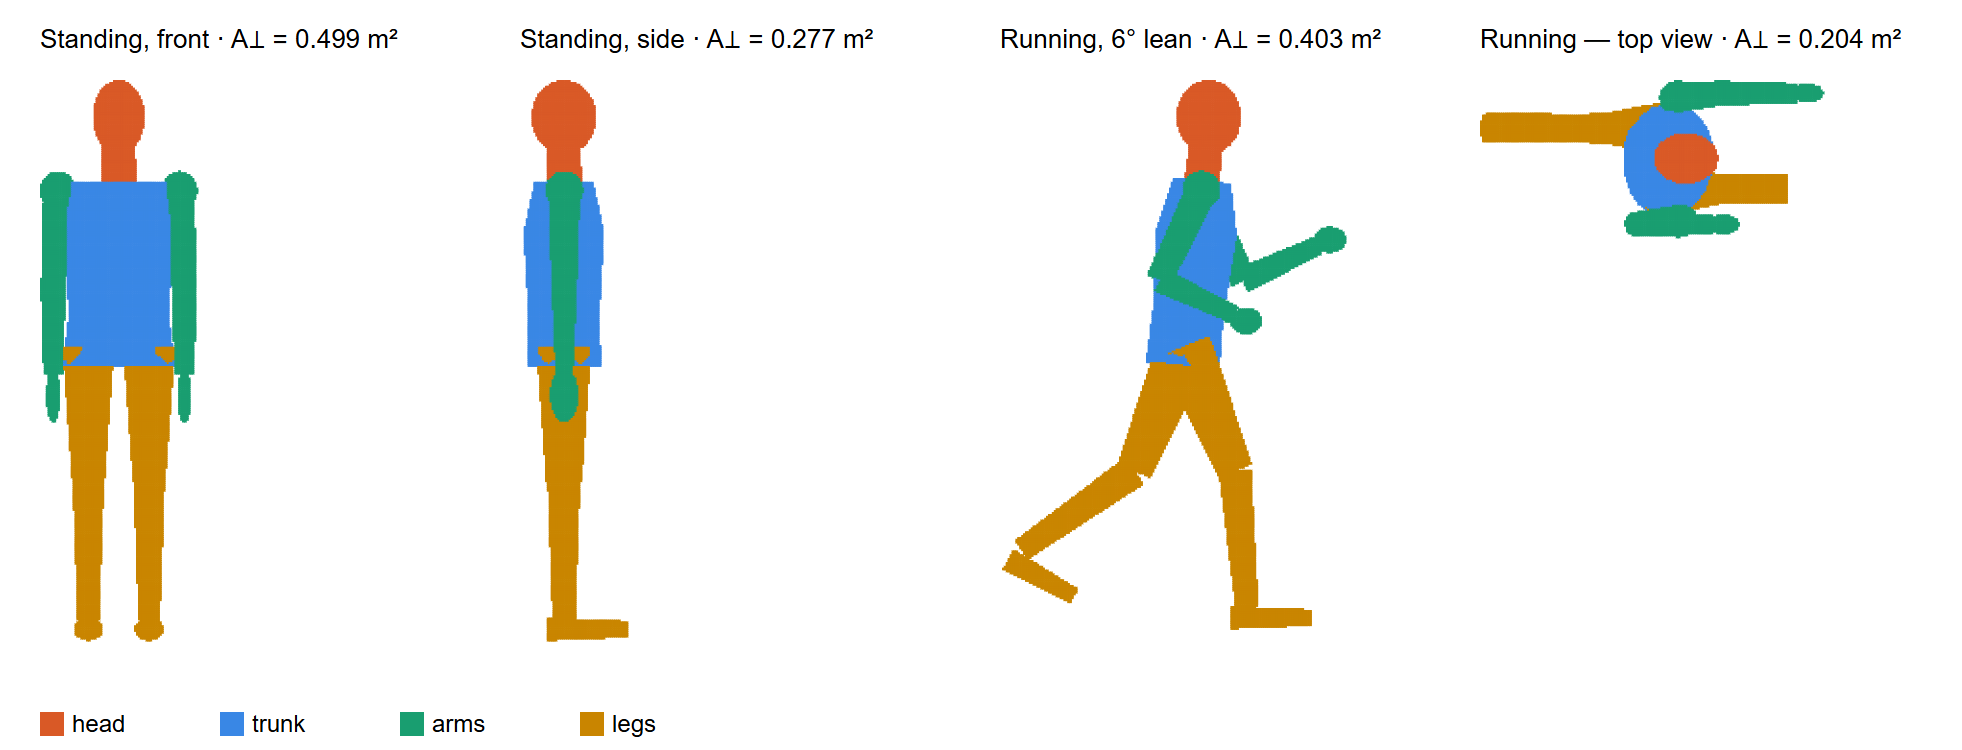
\includegraphics[width=\textwidth]{figures/body_poses.png}
\caption{The parametric body, coloured by region, with silhouette areas. Running exposes thighs and forearms to vertical rain, so the top-view silhouette roughly doubles, from \SI{0.10}{m^2} to \SI{0.21}{m^2}.}\label{fig:body}
\end{figure}

\begin{table}[h]\centering
\caption{Box versus human body ($R=\SI{5}{mm/h}$, $D=\SI{2}{mm}$, \SI{200}{m}; mL), with the human total split by region.}\label{tab:body}
\begin{tabular}{lccccc}\toprule
Wind & $v$ (m/s) & box & human & human/box & head/trunk/arms/legs\\\midrule
Still air & 1.4 & 55.7 & 36.5 & 0.66 & 5.1/14.0/6.7/10.8\\
Still air & 3.3 & 42.9 & 24.6 & 0.57 & 2.6/9.3/6.4/6.3\\
Headwind 3 m/s & 1.4 & 127.3 & 80.4 & 0.63 & 7.6/31.4/15.5/25.9\\
Headwind 3 m/s & 3.3 & 73.2 & 40.6 & 0.55 & 3.9/16.5/8.4/11.8\\
Tailwind 2 m/s & 1.4 & 36.6 & 20.6 & 0.56 & 4.9/9.5/4.6/1.6\\
Tailwind 2 m/s & 3.3 & 22.6 & 18.2 & 0.80 & 2.1/4.4/5.5/6.2\\
Tailwind 5 m/s & 1.4 & 108.2 & 63.8 & 0.59 & 6.8/26.8/13.0/17.2\\
Tailwind 5 m/s & 3.3 & 26.7 & 20.3 & 0.76 & 2.3/7.8/4.8/5.3\\
Crosswind 3 m/s & 1.4 & 95.5 & 47.6 & 0.50 & 7.0/15.3/8.8/16.5\\
Crosswind 3 m/s & 3.3 & 59.8 & 29.4 & 0.49 & 3.3/8.2/6.6/11.3\\\bottomrule
\end{tabular}
\end{table}

In Table~\ref{tab:body} the human collects 50--80\% of the box's water. Crosswind gives the largest reduction, because a real body is much narrower side-on than a box of the same depth. The lean matters less than one might expect: at \SI{3.3}{m/s}, going from $0^\circ$ to $15^\circ$ changes the catch by $-17\%$ in still air and $-11\%$ in a headwind, and by $+22\%$ in a \SI{5}{m/s} tailwind, where leaning exposes the back to rain arriving from behind.

\section{Combined estimate}\label{sec:combined}
To combine the human silhouette with aerodynamic deflection, we split the human catch into two parts. The first is what the body would collect with no horizontal relative motion, $K_{\mathrm{vert}}=C\,\Delta L\,v_t\,A_\perp(\hat z)/v$. The second is the excess over it, and only that excess is scaled by $\eta$:
\begin{equation}
K\approx K_{\mathrm{vert}}+\eta\,(K_{\mathrm{human}}-K_{\mathrm{vert}}).
\end{equation}
This split is exact for a box and approximate otherwise. Table~\ref{tab:combined} and Figure~\ref{fig:refined} compare the result with the box model.

\begin{table}[h]\centering
\caption{Box model versus the combined estimate (human body, Marshall--Palmer rain at \SI{5}{mm/h}, airflow), \SI{200}{m}, in mL. The best pace is found by scanning 0.6--8 m/s.}\label{tab:combined}
\begin{tabular}{lcccc}\toprule
Wind & box walk/run & combined walk/run & box best & combined best\\\midrule
Still air & 55.7/42.9 & 32.6/23.6 & max $\to$ 37.3 & max $\to$ 19.0\\
Headwind 3 m/s & 127.3/73.2 & 74.1/38.8 & max $\to$ 49.8 & max $\to$ 25.6\\
Tailwind 2 m/s & 36.6/22.6 & 20.3/17.9 & 2.0 m/s $\to$ 15.6 & 2.1 m/s $\to$ 13.4\\
Tailwind 5 m/s & 108.2/26.7 & 58.7/19.6 & 5.0 m/s $\to$ 6.2 & 7.9 m/s $\to$ 8.6\\
Crosswind 3 m/s & 95.5/59.8 & 44.0/28.2 & max $\to$ 44.3 & max $\to$ 19.5\\\bottomrule
\end{tabular}
\end{table}

\begin{figure}[h]\centering
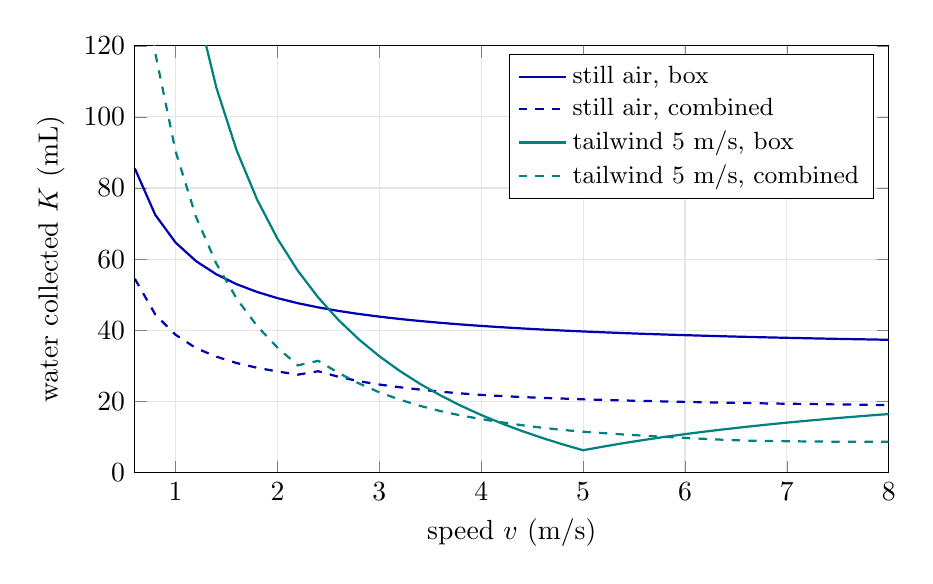
\begin{tikzpicture}
\begin{axis}[width=0.92\textwidth,height=7cm,xmin=0.6,xmax=8,ymin=0,ymax=120,
  xlabel={speed $v$ (m/s)},ylabel={water collected $K$ (mL)},grid=major,grid style={gray!20},
  legend style={font=\small,at={(0.98,0.98)},anchor=north east,cells={anchor=west}}]
\addplot[blue!70!black,thick] coordinates {(0.6,85.49) (0.8,72.47) (1.0,64.66) (1.2,59.45) (1.4,55.73) (1.6,52.94) (1.8,50.77) (2.0,49.03) (2.2,47.61) (2.4,46.43) (2.6,45.43) (2.8,44.57) (3.0,43.83) (3.2,43.17) (3.4,42.60) (3.6,42.09) (3.8,41.63) (4.0,41.22) (4.2,40.85) (4.4,40.51) (4.6,40.20) (4.8,39.92) (5.0,39.66) (5.2,39.42) (5.4,39.20) (5.6,38.99) (5.8,38.80) (6.0,38.62) (6.2,38.45) (6.4,38.29) (6.6,38.14) (6.8,38.00) (7.0,37.87) (7.2,37.75) (7.4,37.63) (7.6,37.52) (7.8,37.42) (8.0,37.31)};
\addlegendentry{still air, box}
\addplot[blue!70!black,thick,dashed] coordinates {(0.6,54.46) (0.8,44.45) (1.0,38.72) (1.2,34.97) (1.4,32.57) (1.6,30.77) (1.8,29.44) (2.0,28.41) (2.2,27.51) (2.4,28.47) (2.6,26.90) (2.8,25.67) (3.0,24.73) (3.2,23.97) (3.4,23.30) (3.6,22.72) (3.8,22.23) (4.0,21.82) (4.2,21.49) (4.4,21.21) (4.6,20.97) (4.8,20.79) (5.0,20.57) (5.2,20.41) (5.4,20.24) (5.6,20.12) (5.8,19.97) (6.0,19.85) (6.2,19.73) (6.4,19.62) (6.6,19.52) (6.8,19.42) (7.0,19.33) (7.2,19.26) (7.4,19.17) (7.6,19.10) (7.8,19.03) (8.0,18.97)};
\addlegendentry{still air, combined}
\addplot[teal,thick] coordinates {(0.6,297.08) (0.8,214.46) (1.0,164.88) (1.2,131.84) (1.4,108.23) (1.6,90.52) (1.8,76.75) (2.0,65.74) (2.2,56.72) (2.4,49.21) (2.6,42.86) (2.8,37.41) (3.0,32.69) (3.2,28.56) (3.4,24.91) (3.6,21.67) (3.8,18.77) (4.0,16.16) (4.2,13.80) (4.4,11.66) (4.6,9.70) (4.8,7.90) (5.0,6.25) (5.2,7.29) (5.4,8.26) (5.6,9.16) (5.8,10.00) (6.0,10.78) (6.2,11.51) (6.4,12.19) (6.6,12.83) (6.8,13.44) (7.0,14.01) (7.2,14.55) (7.4,15.06) (7.6,15.54) (7.8,16.00) (8.0,16.43)};
\addlegendentry{tailwind 5 m/s, box}
\addplot[teal,thick,dashed] coordinates {(0.6,164.00) (0.8,118.00) (1.0,90.31) (1.2,71.91) (1.4,58.73) (1.6,48.87) (1.8,41.18) (2.0,35.11) (2.2,30.12) (2.4,31.40) (2.6,27.96) (2.8,25.05) (3.0,22.54) (3.2,20.49) (3.4,18.74) (3.6,17.25) (3.8,16.03) (4.0,15.01) (4.2,14.11) (4.4,13.29) (4.6,12.57) (4.8,11.97) (5.0,11.46) (5.2,11.07) (5.4,10.68) (5.6,10.34) (5.8,10.02) (6.0,9.72) (6.2,9.43) (6.4,9.17) (6.6,8.96) (6.8,8.86) (7.0,8.80) (7.2,8.72) (7.4,8.67) (7.6,8.64) (7.8,8.61) (8.0,8.62)};
\addlegendentry{tailwind 5 m/s, combined}
\end{axis}
\end{tikzpicture}
\caption{Box model (solid) versus the combined estimate (dashed). The step near \SI{2.2}{m/s} is the walk--run posture switch. With a realistic running body, the sharp tailwind minimum at $v=U_x$ flattens.}\label{fig:refined}
\end{figure}

Three findings stand out.
\begin{enumerate}
\item \emph{Absolute amounts fall by 20--55\%.} Most of the reduction comes from the smaller frontal silhouette; airflow removes a further 5--15\% in moderate rain.
\item \emph{Running still helps in still air and in headwinds,} by about the same proportion as in the box model.
\item \emph{The tailwind rule survives moderate winds but softens in strong ones.} With a \SI{2}{m/s} tailwind the best pace is still the wind speed. With a \SI{5}{m/s} tailwind, a runner who overtakes the rain meets it almost vertically, and the forward thigh and forearms already shade the chest from that direction. Overtaking therefore costs little, while the running pose's larger exposure to vertical rain (Figure~\ref{fig:body}) favours going faster still. The box exaggerates the penalty for overtaking because its front face is fully exposed.
\end{enumerate}

\section{A field experiment}\label{sec:exp}
The central prediction, the dip at $v=U_x$, can be tested with three identical flat absorbent pads of area $A$: one on a cap facing up, one on the chest facing forward and one on the back facing backward. For flat pads,
\begin{equation}
m_{\mathrm{top}}=\rho C A v_t T,\qquad m_{\mathrm{front}}=\rho C A\,\eta\max(0,v-U_x)\,T,\qquad m_{\mathrm{back}}=\rho C A\,\eta\max(0,U_x-v)\,T,
\end{equation}
so the ratios
\begin{equation}
\frac{m_{\mathrm{front}}}{m_{\mathrm{top}}}=k\max(0,v-U_x),\qquad \frac{m_{\mathrm{back}}}{m_{\mathrm{top}}}=k\max(0,U_x-v),\qquad k=\frac{\eta}{v_t},
\end{equation}
do not depend on rain intensity, pad area or trial duration. The top pad is a rain gauge that travels with the walker. A V-shaped dip of the ratios to zero at the anemometer's wind speed confirms the model. The slope $k$ is a field measurement of $\eta/v_t$, and so, with $v_t$ known, of the aerodynamic efficiency itself.

The protocol (\texttt{experiment/PROTOCOL.md}) uses a \SI{100}{m} downwind course and $20\times20$\,cm pads weighed in sealed bags on a \SI{0.01}{g} scale. It covers nine paces from 0.8 to \SI{5}{m/s} in random order, plus extra trials near the wind speed. The analysis script fits $U_x$ and $k$ by least squares and compares the fit with a wind-blind alternative ($m_{\mathrm{front}}/m_{\mathrm{top}}\propto v$, back dry) by AIC, with bootstrap confidence intervals.

We ran the protocol on synthetic campaigns generated from the model, adding trial-to-trial gusts, rain variability, scale noise and handling losses (Table~\ref{tab:power}). Under typical conditions, a single repeat of nine trials locates a \SI{2}{m/s} tailwind to within about $\pm\SI{0.3}{m/s}$. Under pessimistic conditions, three repeats (27 trials, one afternoon) are needed to detect the dip reliably.

\begin{table}[h]\centering
\caption{Simulated power of the field experiment (40 synthetic campaigns per row, \SI{2}{m/s} tailwind). Typical: gusts $\pm\SI{0.35}{m/s}$, rain $\pm30\%$, handling $\pm4\%$. Pessimistic: gusts $\pm\SI{0.8}{m/s}$, rain $\pm50\%$, handling $\pm12\%$.}\label{tab:power}
\begin{tabular}{lcccc}\toprule
Conditions & trials & median $|U_x$ error$|$ & 95\% CI width & dip detected\\\midrule
Typical & 9 & 0.07 m/s & 0.58 m/s & 100\%\\
Typical & 18 & 0.06 m/s & 0.35 m/s & 100\%\\
Pessimistic & 9 & 0.23 m/s & 1.87 m/s & 43\%\\
Pessimistic & 27 & 0.15 m/s & 0.75 m/s & 95\%\\
Pessimistic & 45 & 0.12 m/s & 0.57 m/s & 100\%\\\bottomrule
\end{tabular}
\end{table}

\section{Limitations and future work}
\begin{itemize}
\item \emph{Airflow} is two-dimensional potential flow around horizontal sections. A three-dimensional simulation with a turbulence model (RANS or LES) around the mesh would quantify the wake and the flow over the head, and how far the true $\eta$ exceeds our lower bound.
\item \emph{Posture.} The lean schedule and running pose are modelled, not measured. Motion-capture data would replace them and add the time-varying limb positions over a stride.
\item \emph{Body.} The parametric body represents one adult man. Loading 3D scans of other body types is supported but has not been done.
\item \emph{Rain.} Gusts, splashing, clothing absorption and run-off are not modelled. Over long distances clothing saturates, after which the water collected is no longer the water retained.
\item \emph{Validation.} The field experiment of Section~\ref{sec:exp} has been designed and simulated, not performed.
\end{itemize}

\begin{thebibliography}{99}
\bibitem{holden1995} J.~J.~Holden, S.~E.~Belcher, \'A.~Horv\'ath, I.~Pytte, ``Raindrops keep falling on my head,'' \emph{Weather} \textbf{50}, 367--370 (1995).
\bibitem{ehrmann2011} A.~Ehrmann, T.~Blachowicz, ``Walking or running in the rain---a simple derivation of a general solution,'' \emph{Eur.\ J.\ Phys.} \textbf{32}, 355--361 (2011).
\bibitem{bocci2012} F.~Bocci, ``Whether or not to run in the rain,'' \emph{Eur.\ J.\ Phys.} \textbf{33}, 1321--1332 (2012).
\bibitem{gunn1949} R.~Gunn, G.~D.~Kinzer, ``The terminal velocity of fall for water droplets in stagnant air,'' \emph{J.\ Meteor.} \textbf{6}, 243--248 (1949).
\bibitem{atlas1973} D.~Atlas, R.~C.~Srivastava, R.~S.~Sekhon, ``Doppler radar characteristics of precipitation at vertical incidence,'' \emph{Rev.\ Geophys.\ Space Phys.} \textbf{11}, 1--35 (1973).
\bibitem{pugh1971} L.~G.~C.~E.~Pugh, ``The influence of wind resistance in running and walking and the mechanical efficiency of work against horizontal or vertical forces,'' \emph{J.\ Physiol.} \textbf{213}, 255--276 (1971).
\bibitem{marshall1948} J.~S.~Marshall, W.~M.~Palmer, ``The distribution of raindrops with size,'' \emph{J.\ Meteor.} \textbf{5}, 165--166 (1948).
\end{thebibliography}
\end{document}
